
\providecommand{\Cat}{\mathcal{C}at}
\providecommand{\sSet}{s\mathcal{S}et}

\section{\trChangeOfBase}\label{sec:change-of-base}

「\trChangeOfBase」（change of base）最初由 Eilenberg 与 Kelly 在 \cite{bib41}
中考虑，指的是这样一种系统性的程序：把对一个范畴 $\mathcal{V}$ 的富集转换为对
另一个范畴 $\mathcal{W}$ 的富集。\cref{cor:vcat-two-category}指出：对一个%
\trCartesianClosed{}范畴 $\mathcal{V}$，存在一个由 $\mathcal{V}$-范畴、
$\mathcal{V}$-函子与 $\mathcal{V}$-自然变换组成的 2-\trCategory{}
$\mathcal{V}\text{-}\Cat$。第一个主要结果即\cref{prop:change-of-base-2-functor}，
它给出这样的条件：使一个介于\trCartesianClosed{}范畴之间的\trFunctor{}
$T\colon\mathcal{V}\to\mathcal{W}$ 诱导一个换基 2-\trFunctor{}
$T_{*}\colon\mathcal{V}\text{-}\Cat\to\mathcal{W}\text{-}\Cat$。

我们在此工作的语境不如 Eilenberg 与 Kelly 所考虑的那般一般——我们的基范畴是%
\trCartesianClosed{}，而他们的则是封闭对称幺半的——于是我们采取一条覆盖
我们全部例子且更易于解释的捷径。一般地，造出一个换基 2-函子所需要的，只是
对称幺半范畴之间的一个\emph{松幺半函子}（lax monoidal functor）；但我们在%
\trCartesianClosed{}范畴之间遇到的松幺半函子事实上都保持有限积，于是我们便
满足于把这一情形下的结果阐明出来。

回忆：介于\trCartesianClosed{}范畴之间的一个\trFunctor{}
$T\colon\mathcal{V}\to\mathcal{W}$ \textbf{保持有限积}（preserves finite
products），恰当对任何 $u$，$v\in\mathcal{V}$ 所定义的自然映射
\[ T(u\times v)\xRightarrow{\sim}Tu\times Tv
   \qquad\text{以及}\qquad
   T1\xRightarrow{\sim}1 \]
是\trIsomorphism。例如：

\begin{example}\label{exa:underlying-set-product-preserving}
由于可表示函子保持积，对任何\trCartesianClosed{}范畴 $\mathcal{V}$，底集函子
$(-)_{0}\colon\mathcal{V}\to\mathcal{S}et$ 是保持积的。
\end{example}

\begin{example}\label{exa:coproduct-functor-product-preserving}
在一个\trCartesianClosed{}范畴 $\mathcal{V}$ 中，有限积对任意\trCoproduct{}%
分配。特别地，对任何集合 $X$ 与 $Y$，在\trTerminal{}对象 $1$ 的诸%
\trCoproduct{}之间存在一个\trIsomorphism
\[ \coprod_{X\times Y}1\cong\bigl(\coprod_{X}1\bigr)\times
   \bigl(\coprod_{Y}1\bigr) \]
这就证明了\trFunctor
\[ \mathcal{S}et\xrightarrow{\ \coprod_{-}1\ }\mathcal{V} \]
是保持有限积的。
\end{example}

一个保持有限积的\trFunctor{}可以按下述方式用来更换基。

\begin{proposition}\label{prop:change-of-base-2-functor}
一个介于\trCartesianClosed{}范畴之间的、保持有限积的\trFunctor{}
$T\colon\mathcal{V}\to\mathcal{W}$ 诱导一个换基 2-\trFunctor
\[ \mathcal{V}\text{-}\Cat\xrightarrow{\ T_{*}\ }\mathcal{W}\text{-}\Cat. \]
\end{proposition}

沿这些路线的一个早期观察首先表述于 \cite[II.6.3]{bib41}，其证明留给读者。我们
采取同样的策略，把诸图表追索（diagram chase）留给读者或 \cite[4.2.4]{bib31}，
而只给出换基 2-函子的构造——这才是要紧之处。

\begin{proof}
设 $\mathcal{C}$ 是一个 $\mathcal{V}$-范畴，并定义一个 $\mathcal{W}$-范畴
$T_{*}\mathcal{C}$：它与 $\mathcal{C}$ 有相同的对象，其映射对象（mapping
objects）为 $T_{*}\mathcal{C}(x,y)\coloneqq T\mathcal{C}(x,y)$。复合与单位映射
由诸复合映射
\[ T\mathcal{C}(y,z)\times T\mathcal{C}(x,y)
   \xrightarrow{\ \cong\ }
   T\bigl(\mathcal{C}(y,z)\times\mathcal{C}(x,y)\bigr)
   \xrightarrow{\ T\circ\ }T\mathcal{C}(x,z) \]
\[ 1\xrightarrow{\ \cong\ }T1\xrightarrow{\ T\mathrm{id}_{x}\ }T\mathcal{C}(x,x) \]
给出，其中用到了把一个保持有限积的\trFunctor{}施于一个有限积时所产生的那些
自然映射之逆。一幅直截的图表追索即可验证 $T_{*}\mathcal{C}$ 是一个
$\mathcal{W}$-范畴。

若 $F\colon\mathcal{C}\to\mathcal{D}$ 是一个 $\mathcal{V}$-函子，则我们定义一
个 $\mathcal{W}$-函子 $T_{*}F\colon T_{*}\mathcal{C}\to T_{*}\mathcal{D}$：它
在对象上的作用为 $c\in\mathcal{C}\mapsto Fc\in\mathcal{D}$，而在箭头上的内部
作用则由
\[ T\mathcal{C}(x,y)\xrightarrow{\ TF_{x,y}\ }T\mathcal{D}(Fx,Fy) \]
定义。同样，一幅直截的图表追索即可验证 $T_{*}F$ 是 $\mathcal{W}$-函子性的。
由这个定义显而易见：$T_{*}(GF)=T_{*}G\cdot T_{*}F$。

最后，设 $\alpha\colon F\Rightarrow G$ 是介于 $\mathcal{V}$-函子
$F,G\colon\mathcal{C}\to\mathcal{D}$ 之间的一个 $\mathcal{V}$-自然变换，并定
义一个 $\mathcal{W}$-自然变换 $T_{*}\alpha\colon T_{*}F\Rightarrow T_{*}G$，
其分量为
\[ 1\xrightarrow{\ \cong\ }T1\xrightarrow{\ T\alpha_{c}\ }T\mathcal{D}(Fc,Gc) \]
再一幅直截的图表追索即可验证 $T_{*}\alpha$ 是 $\mathcal{W}$-自然的。

尚须验证：这一指派对富集\trNaturalTransformation{}的水平复合与竖直复合都是
函子性的。查\cref{def:vertical-horizontal-composites}可见，$T_{*}(\beta\cdot\alpha)$
的分量由下方的顶行复合定义，而 $T_{*}\alpha$ 与 $T_{*}\beta\colon T_{*}G\Rightarrow T_{*}H$
的竖直复合之分量的定义即底行复合：
\begin{center}
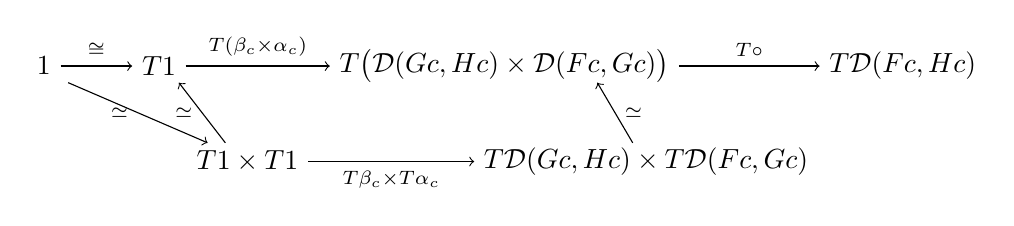
\begin{tikzpicture}[x=1.6em,y=1.5em]
  \node (a1) at (0,2.3) {$1$};
  \node (a2) at (2.6,2.3) {$T1$};
  \node (a3) at (10.4,2.3)
    {$T\bigl(\mathcal{D}(Gc,Hc)\times\mathcal{D}(Fc,Gc)\bigr)$};
  \node (a4) at (19.4,2.3) {$T\mathcal{D}(Fc,Hc)$};
  \draw[->] (a1) -- node[above]{$\scriptstyle\cong$} (a2);
  \draw[->] (a2) -- node[above]{$\scriptstyle T(\beta_{c}\times\alpha_{c})$} (a3);
  \draw[->] (a3) -- node[above]{$\scriptstyle T\circ$} (a4);
  \node (b1) at (4.6,0) {$T1\times T1$};
  \node (b2) at (13.6,0)
    {$T\mathcal{D}(Gc,Hc)\times T\mathcal{D}(Fc,Gc)$};
  \draw[->] (b1) -- node[below]{$\scriptstyle T\beta_{c}\times T\alpha_{c}$} (b2);
  \draw[->] (0.55,1.9) -- node[left,pos=0.5]{$\scriptstyle\simeq$} (3.7,0.45);
  \draw[->] (4.1,0.45) -- node[left]{$\scriptstyle\simeq$} (3.05,1.9);
  \draw[->] (13.3,0.45) -- node[right]{$\scriptstyle\simeq$} (12.5,1.9);
\end{tikzpicture}
\end{center}
该方块由\trIsomorphism{} $T(u\times v)\cong Tu\times Tv$ 的自然性而交换，而
三角形之所以交换，是因为 $1$ 是\trTerminal{}对象，于是所示诸\trIsomorphism{}%
之逆构成一个交换三角形。水平复合之函子性的论证类似。
\end{proof}

\begin{remark}\label{rem:change-of-base-2-functorial}
事实上，「换基」这一程序 $\mathcal{V}\mapsto\mathcal{V}\text{-}\Cat$
\emph{本身}就是一支 2-\trFunctor：从由\trCartesianClosed{}范畴、保持有限积的%
\trFunctor{}与\trNaturalTransformation{}构成的 2-\trCategory，到由 2-范畴、
2-\trFunctor{}与 2-自然变换构成的 2-\trCategory。讨论与证明见
\cite[\S\,4.3]{bib31}。
\end{remark}

作为\cref{rem:change-of-base-2-functorial}之 2-函子性的一个直接推论：

\begin{proposition}\label{prop:change-of-base-2-adjunction}
任何一支介于\trCartesianClosed{}范畴之间、其左伴随保持有限积的\trAdjunction，
都诱导一个换基 2-伴随
\begin{center}
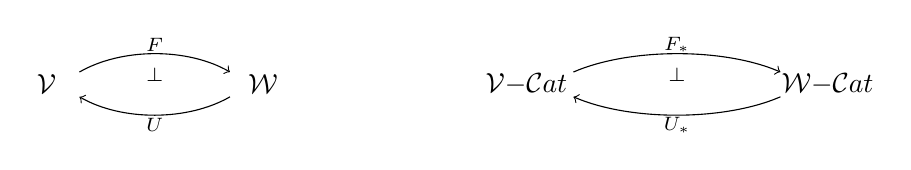
\begin{tikzpicture}[x=1.7em,y=1.4em]
  \node (v) at (0,0) {$\mathcal{V}$};
  \node (w) at (4.6,0) {$\mathcal{W}$};
  \draw[->] (0.7,0.32) .. controls (1.6,0.95) and (3.0,0.95) .. (3.9,0.32);
  \node at (2.3,1.02) {$\scriptstyle F$};
  \node at (2.3,0.25) {$\scriptstyle\bot$};
  \draw[->] (3.9,-0.32) .. controls (3.0,-0.95) and (1.6,-0.95) .. (0.7,-0.32);
  \node at (2.3,-1.05) {$\scriptstyle U$};
  \node at (7.4,0) {$\scriptstyle\rightsquigarrow$};
  \begin{scope}[shift={(10.2,0)}]
    \node (vc) at (0,0) {$\mathcal{V}\text{-}\Cat$};
    \node (wc) at (6.4,0) {$\mathcal{W}\text{-}\Cat$};
    \draw[->] (1.0,0.32) .. controls (2.2,0.95) and (4.2,0.95) .. (5.4,0.32);
    \node at (3.2,1.02) {$\scriptstyle F_{*}$};
    \node at (3.2,0.25) {$\scriptstyle\bot$};
    \draw[->] (5.4,-0.32) .. controls (4.2,-0.95) and (2.2,-0.95) .. (1.0,-0.32);
    \node at (3.2,-1.05) {$\scriptstyle U_{*}$};
  \end{scope}
\end{tikzpicture}
\end{center}
\end{proposition}

\begin{proof}
当然，右伴随总是保持积的，故\trFunctor{}伴随对 $F\dashv U$ 在
\cref{rem:change-of-base-2-functorial}所描述的那个「\trCartesianClosed{}范畴
与保持有限积的\trFunctor」之 2-\trCategory{}中定义一个\trAdjunction。于是，
2-\trFunctor{} $\mathcal{V}\mapsto\mathcal{V}\text{-}\Cat$ 把左侧所示的%
\trAdjunction{}带到右侧所示的\trAdjunction。
\end{proof}

作为一个特例：

\begin{corollary}\label{cor:underlying-free-2-adjunction}
对任何容有\trCoproduct{}的\trCartesianClosed{}范畴 $\mathcal{V}$，取底范畴的
构造与取自由范畴的构造定义一对伴随的 2-\trFunctor
\begin{center}
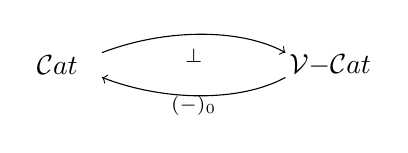
\begin{tikzpicture}[x=1.7em,y=1.4em]
  \node (c) at (0,0) {$\Cat$};
  \node (vc) at (5.8,0) {$\mathcal{V}\text{-}\Cat$};
  \draw[->] (0.95,0.32) .. controls (2.3,0.95) and (3.9,0.95) .. (4.85,0.32);
  \node at (2.9,0.25) {$\scriptstyle\bot$};
  \draw[->] (4.85,-0.32) .. controls (3.9,-0.95) and (2.3,-0.95) .. (0.95,-0.32);
  \node at (2.9,-1.05) {$\scriptstyle(-)_{0}$};
\end{tikzpicture}
\end{center}
\end{corollary}

鉴于\cref{prop:change-of-base-2-adjunction}与随后的诸结果，一支介于%
\trCartesianClosed{}范畴之间、其左伴随保持有限积的\trAdjunction{}提供一个
\textbf{换基伴随}（change-of-base adjunction）。
\cref{prop:change-of-base-2-adjunction}容许沿一支保持有限积的\trAdjunction{}%
的任一伴随作换基，而接下来的一系列结果将揭示：沿右伴随的换基表现要更好一些。

\begin{lemma}\label{lem:finite-product-adjunction-v-enriched}
任何一支由介于\trCartesianClosed{}范畴之间的、保持有限积的诸\trFunctor{}构成
的\trAdjunction
\begin{center}
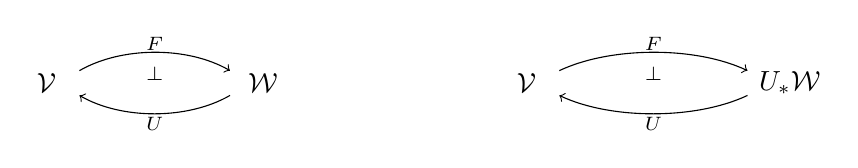
\begin{tikzpicture}[x=1.7em,y=1.4em]
  \node (v) at (0,0) {$\mathcal{V}$};
  \node (w) at (4.6,0) {$\mathcal{W}$};
  \draw[->] (0.7,0.32) .. controls (1.6,0.95) and (3.0,0.95) .. (3.9,0.32);
  \node at (2.3,1.02) {$\scriptstyle F$};
  \node at (2.3,0.25) {$\scriptstyle\bot$};
  \draw[->] (3.9,-0.32) .. controls (3.0,-0.95) and (1.6,-0.95) .. (0.7,-0.32);
  \node at (2.3,-1.05) {$\scriptstyle U$};
  \node at (7.4,0) {$\scriptstyle\rightsquigarrow$};
  \begin{scope}[shift={(10.2,0)}]
    \node (v2) at (0,0) {$\mathcal{V}$};
    \node (uw) at (5.6,0) {$U_{*}\mathcal{W}$};
    \draw[->] (0.7,0.32) .. controls (1.8,0.95) and (3.6,0.95) .. (4.7,0.32);
    \node at (2.7,1.02) {$\scriptstyle F$};
    \node at (2.7,0.25) {$\scriptstyle\bot$};
    \draw[->] (4.7,-0.32) .. controls (3.6,-0.95) and (1.8,-0.95) .. (0.7,-0.32);
    \node at (2.7,-1.05) {$\scriptstyle U$};
  \end{scope}
\end{tikzpicture}
\end{center}
都在诸 $\mathcal{V}$-范畴 $\mathcal{V}$ 与 $U_{*}\mathcal{W}$ 之间定义一个
$\mathcal{V}$-富集\trAdjunction；亦即，存在一个 $\mathcal{V}$-自然%
\trIsomorphism
\[ UW(Fv,w)\cong\mathcal{V}(v,Uw). \]
\end{lemma}

\begin{proof}
$\mathcal{V}$-函子 $U\colon U_{*}\mathcal{W}\to\mathcal{V}$ 的内部作用
$U_{a,b}\colon UW(a,b)\to\mathcal{V}(Ua,Ub)$ 定义为映射
$U\mathrm{ev}\colon UW(a,b)\times Ua\to Ub$ 的转置，后者由把 $U$ 施于
$\mathcal{W}$ 的\trCartesianClosed{}伴随之余单位而得。交换方块
\eqref{eq:composition-transpose-square}提供了这个映射的 $\mathcal{V}$-函子性。

由 $U\colon U_{*}\mathcal{W}\to\mathcal{V}$ 的 $\mathcal{V}$-函子性，映射
\[ UW(Fv,w)\xrightarrow{\ U_{Fv,w}\ }\mathcal{V}(UFv,Uw)
   \xrightarrow{\ -\circ\eta_{v}\ }\mathcal{V}(v,Uw) \]
对一切 $v\in\mathcal{V}$ 都在 $w\in U_{*}\mathcal{W}$ 中是 $\mathcal{V}$-自然
的。由\cref{rem:vleft-adjoint-representability}，为给 $F$ 构造一个相容的
$\mathcal{V}$-富集，只需证明这个映射是 $\mathcal{V}$ 中的一个\trIsomorphism。

我们通过构造一个显式的逆来做到这一点，即
\[ \mathcal{V}(v,Uw)\xrightarrow{\ \eta\ }UF\mathcal{V}(v,Uw)
   \xrightarrow{\ U(F_{v,Uw})\ }UW(Fv,FUw)
   \xrightarrow{\ \varepsilon_{w}\circ-\ }UW(Fv,w) \]
其中中间那个映射定义为：把非富集\trFunctor{} $U$ 施于来自 $\mathcal{W}$-函子
$F\colon F_{*}\mathcal{V}\to\mathcal{W}$ 的作用映射，而该 $\mathcal{W}$-函子
的定义方式与 $\mathcal{V}$-函子 $U\colon U_{*}\mathcal{W}\to\mathcal{V}$ 类似。

这两个映射互逆的证明涉及一对图表追索，其中第一幅表明：右上复合约化到左下复合，
而后者是恒同：
\begin{center}
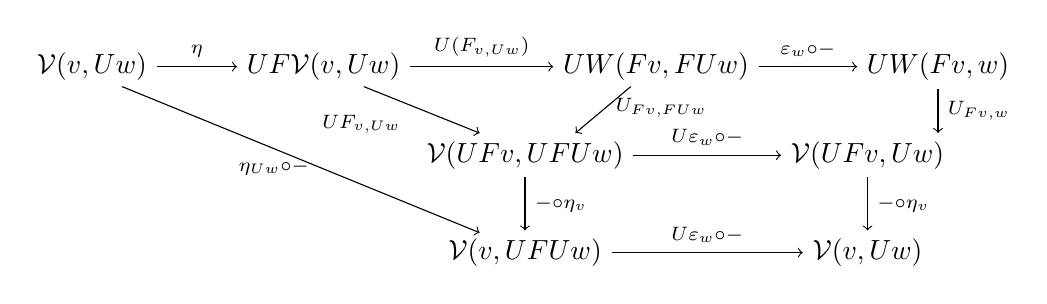
\begin{tikzpicture}[x=1.82em,y=1.6em]
  \node (a) at (0,3.2) {$\mathcal{V}(v,Uw)$};
  \node (b) at (4.6,3.2) {$UF\mathcal{V}(v,Uw)$};
  \node (c) at (11.2,3.2) {$UW(Fv,FUw)$};
  \node (d) at (16.8,3.2) {$UW(Fv,w)$};
  \draw[->] (a) -- node[above]{$\scriptstyle\eta$} (b);
  \draw[->] (b) -- node[above]{$\scriptstyle U(F_{v,Uw})$} (c);
  \draw[->] (c) -- node[above]{$\scriptstyle\varepsilon_{w}\circ-$} (d);
  \node (e) at (8.6,1.2) {$\mathcal{V}(UFv,UFUw)$};
  \node (f) at (15.4,1.2) {$\mathcal{V}(UFv,Uw)$};
  \draw[->] (e) -- node[above]{$\scriptstyle U\varepsilon_{w}\circ-$} (f);
  \draw[->] (10.7,2.75) -- node[right,pos=0.45]{$\scriptstyle U_{Fv,FUw}$} (9.6,1.7);
  \draw[->] (16.8,2.7) -- node[right]{$\scriptstyle U_{Fv,w}$} (16.8,1.7);
  \draw[->] (5.4,2.75) -- node[below left,pos=0.4]{$\scriptstyle UF_{v,Uw}$} (7.7,1.7);
  \node (g) at (15.4,-1.0) {$\mathcal{V}(v,Uw)$};
  \draw[->] (15.4,0.7) -- node[right]{$\scriptstyle-\circ\eta_{v}$} (15.4,-0.5);
  \node (h) at (8.6,-1.0) {$\mathcal{V}(v,UFUw)$};
  \draw[->] (8.6,0.7) -- node[right]{$\scriptstyle-\circ\eta_{v}$} (8.6,-0.5);
  \draw[->] (h) -- node[above]{$\scriptstyle U\varepsilon_{w}\circ-$} (g);
  \draw[->] (0.6,2.75) -- node[left,pos=0.55]{$\scriptstyle\eta_{Uw}\circ-$} (7.7,-0.55);
\end{tikzpicture}
\end{center}
唯一的微妙之处在于梯形区域的交换性，它表达这样一个事实：$\eta\colon\allowbreak\mathrm{id}_{\mathcal{V}}\Rightarrow UF$
是介于\trCartesianClosed{}范畴之间的、保持积的诸\trFunctor{}之间的一个
\emph{闭自然变换}（closed natural transformation）。该区域之所以交换，是因为
其转置后的图表交换：
\begin{center}
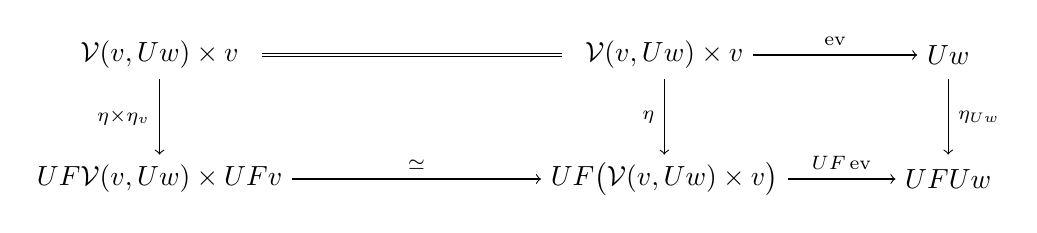
\begin{tikzpicture}[x=1.9em,y=1.6em]
  \node (t1) at (0,1.7) {$\mathcal{V}(v,Uw)\times v$};
  \node (t2) at (9.6,1.7) {$\mathcal{V}(v,Uw)\times v$};
  \node (t3) at (15.0,1.7) {$Uw$};
  \draw[double,double distance=0.6pt] (1.95,1.7) -- (7.65,1.7);
  \draw[->] (t2) -- node[above]{$\scriptstyle\mathrm{ev}$} (t3);
  \node (b1) at (0,-1.1) {$UF\mathcal{V}(v,Uw)\times UFv$};
  \node (b2) at (9.6,-1.1) {$UF\bigl(\mathcal{V}(v,Uw)\times v\bigr)$};
  \node (b3) at (15.0,-1.1) {$UFUw$};
  \draw[->] (b1) -- node[above]{$\scriptstyle\simeq$} (b2);
  \draw[->] (b2) -- node[above]{$\scriptstyle UF\,\mathrm{ev}$} (b3);
  \draw[->] (0,1.15) -- node[left]{$\scriptstyle\eta\times\eta_{v}$} (0,-0.55);
  \draw[->] (9.6,1.15) -- node[left]{$\scriptstyle\eta$} (9.6,-0.55);
  \draw[->] (15.0,1.15) -- node[right]{$\scriptstyle\eta_{Uw}$} (15.0,-0.55);
\end{tikzpicture}
\end{center}
右侧方块由自然性而交换，而左侧方块之所以交换，则是因为介于保持积的诸%
\trFunctor{}之间的任何\trNaturalTransformation{}都自动是一个幺半自然变换
（见\cref{ex:monoidal-functors}）。另一幅图表追索类似。
\end{proof}

\begin{proposition}\label{prop:change-of-base-tensored-cotensored}
给定一支介于\trCartesianClosed{}范畴之间的\trAdjunction
\begin{center}
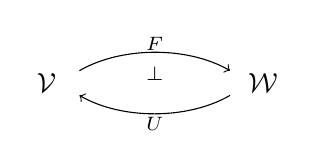
\begin{tikzpicture}[x=1.7em,y=1.4em]
  \node (v) at (0,0) {$\mathcal{V}$};
  \node (w) at (4.6,0) {$\mathcal{W}$};
  \draw[->] (0.7,0.32) .. controls (1.6,0.95) and (3.0,0.95) .. (3.9,0.32);
  \node at (2.3,1.02) {$\scriptstyle F$};
  \node at (2.3,0.25) {$\scriptstyle\bot$};
  \draw[->] (3.9,-0.32) .. controls (3.0,-0.95) and (1.6,-0.95) .. (0.7,-0.32);
  \node at (2.3,-1.05) {$\scriptstyle U$};
\end{tikzpicture}
\end{center}
其左伴随保持有限积。若 $\mathcal{C}$ 作为 $\mathcal{W}$-范畴是余/张量化的，
则 $U_{*}\mathcal{C}$ 作为 $\mathcal{V}$-范畴是余/张量化的，其中 $c\in\mathcal{C}$
经 $v\in\mathcal{V}$ 的余/张量由
\[ v\otimes c\coloneqq Fv\otimes c
   \qquad\text{以及}\qquad
   c^{v}\coloneqq c^{Fv} \]
定义。
\end{proposition}

\begin{proof}
设 $\mathcal{C}$ 作为 $\mathcal{W}$-范畴容有余张量。为验证 $U_{*}\mathcal{C}$
作为 $\mathcal{V}$-范畴容有余张量，我们必须供给一个居于 $\mathcal{V}$ 之中、
在 $x$ 上 $\mathcal{V}$-自然的\trIsomorphism
\[ U\mathcal{C}(x,c^{Fv})\cong\bigl(U\mathcal{C}(x,c)\bigr)^{v} \]
由富集\trYonedaLemma，我们可以从一个在 $u\in\mathcal{V}$ 上 $\mathcal{V}$-自
然的\trIsomorphism
\[ \mathcal{V}\bigl(u,U\mathcal{C}(x,c^{Fv})\bigr)
   \cong\mathcal{V}\bigl(u,\bigl(U\mathcal{C}(x,c)\bigr)^{v}\bigr) \]
中提取出这个\trIsomorphism。为此，把\cref{lem:finite-product-adjunction-v-enriched}
的诸 $\mathcal{V}$-自然\trIsomorphism、源自 $\mathcal{V}$ 与 $\mathcal{W}$%
\footnote{原书此处印作「on $\mathcal{V}$ and on $U_{*}\mathcal{W}$」；按下方
同构链中 $UW\bigl(Fu,\mathcal{C}(x,c)^{Fv}\bigr)\cong UW\bigl(Fu\times Fv,\mathcal{C}(x,c)\bigr)$ 一步系施用 $\mathcal{W}$ 的%
\trCartesianClosed{}结构，而 $U_{*}\mathcal{W}$ 系 $\mathcal{V}$-范畴、本无
笛卡尔封闭结构可言，疑为 $\mathcal{W}$ 之误，此处径改。——译者注}
上\trCartesianClosed{}结构的那些富集自然\trIsomorphism、以及刻画 $\mathcal{C}$
上的余张量并表达 $F$ 保持二元\trProduct{}这一事实的那些\trIsomorphism{}复合%
起来，便有：
\begin{align*}
\mathcal{V}\bigl(u,U\mathcal{C}(x,c^{Fv})\bigr)
  &\cong UW\bigl(Fu,\mathcal{C}(x,c^{Fv})\bigr)
   \cong UW\bigl(Fu,\mathcal{C}(x,c)^{Fv}\bigr)\\
  &\cong UW\bigl(Fu\times Fv,\mathcal{C}(x,c)\bigr)
   \cong UW\bigl(F(u\times v),\mathcal{C}(x,c)\bigr)\\
  &\cong\mathcal{V}\bigl(u\times v,U\mathcal{C}(x,c)\bigr)
   \cong\mathcal{V}\bigl(u,\bigl(U\mathcal{C}(x,c)\bigr)^{v}\bigr).
\end{align*}
\end{proof}

这套换基理论，从富集范畴的复合名词视角看固然很好，但形容词的观点还会生出一层
额外的关切。若保持有限积的\trFunctor{} $T\colon\mathcal{V}\to\mathcal{W}$ 在
自然\trIsomorphism{}的意义下与 $\mathcal{V}$ 和 $\mathcal{W}$ 的底集函子交换，
则由\cref{rem:change-of-base-2-functorial}的 2-函子性，换基 2-函子
$T_{*}\colon\mathcal{V}\text{-}\Cat\to\mathcal{W}\text{-}\Cat$ 也在自然%
\trIsomorphism{}的意义下保持诸底范畴。这特别地发生于如下设定中。

\begin{lemma}\label{lem:change-of-base-underlying-categories}
考虑一支介于\trCartesianClosed{}范畴之间的、保持有限积的\trAdjunction：
\begin{center}
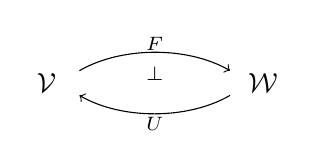
\begin{tikzpicture}[x=1.7em,y=1.4em]
  \node (v) at (0,0) {$\mathcal{V}$};
  \node (w) at (4.6,0) {$\mathcal{W}$};
  \draw[->] (0.7,0.32) .. controls (1.6,0.95) and (3.0,0.95) .. (3.9,0.32);
  \node at (2.3,1.02) {$\scriptstyle F$};
  \node at (2.3,0.25) {$\scriptstyle\bot$};
  \draw[->] (3.9,-0.32) .. controls (3.0,-0.95) and (1.6,-0.95) .. (0.7,-0.32);
  \node at (2.3,-1.05) {$\scriptstyle U$};
\end{tikzpicture}
\end{center}
那么，沿右伴随的换基尊重诸底范畴：
\begin{center}
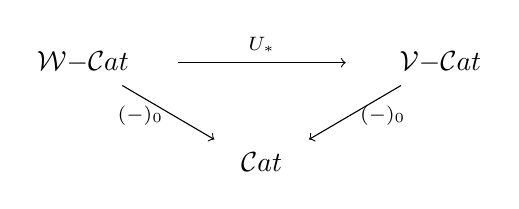
\begin{tikzpicture}[x=1.9em,y=1.5em]
  \node (wc) at (0,1.3) {$\mathcal{W}\text{-}\Cat$};
  \node (vc) at (6.8,1.3) {$\mathcal{V}\text{-}\Cat$};
  \draw[->] (1.8,1.3) -- node[above]{$\scriptstyle U_{*}$} (5.0,1.3);
  \node (cat) at (3.4,-1.1) {$\Cat$};
  \draw[->] (0.75,0.75) -- node[left,pos=0.55]{$\scriptstyle(-)_{0}$} (2.5,-0.55);
  \draw[->] (6.05,0.75) -- node[right,pos=0.55]{$\scriptstyle(-)_{0}$} (4.3,-0.55);
\end{tikzpicture}
\end{center}
\end{lemma}

\begin{proof}
设 $\mathcal{C}$ 是一个 $\mathcal{W}$-范畴。$U_{*}\mathcal{C}$ 的底范畴中从
$x$ 到 $y$ 的 hom-集，同构于 $\mathcal{C}$ 的底范畴中相应的 hom-集
\[ U_{*}\mathcal{C}(x,y)_{0}
   \cong\mathcal{V}\bigl(1,U\mathcal{C}(x,y)\bigr)_{0}
   \cong\mathcal{W}\bigl(F1,\mathcal{C}(x,y)\bigr)_{0}
   \cong\mathcal{W}\bigl(1,\mathcal{C}(x,y)\bigr)_{0}
   \cong\mathcal{C}(x,y)_{0} \]
而且这个\trIsomorphism{}尊重诸底范畴中的复合与单位。于是
$\mathcal{C}_{0}\cong U_{*}\mathcal{C}_{0}$。类似的论证表明：沿 $U$ 的换基
尊重底\trFunctor{}与底\trNaturalTransformation。
\end{proof}

我们以重返第 1 章中的\cref{dig:change-of-base}所预演过的一个例子，来为本章
收尾。

\begin{example}\label{exa:homotopy-nerve-change-of-base}
第 1 章中的\cref{prop:nerve-left-adjoint}的\trAdjunction
\begin{center}
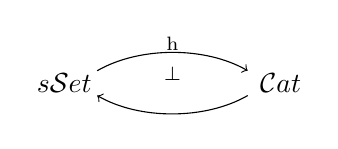
\begin{tikzpicture}[x=1.7em,y=1.4em]
  \node (ss) at (0,0) {$\sSet$};
  \node (ct) at (4.6,0) {$\Cat$};
  \draw[->] (0.7,0.32) .. controls (1.6,0.95) and (3.0,0.95) .. (3.9,0.32);
  \node at (2.3,1.02) {$\scriptstyle\mathrm{h}$};
  \node at (2.3,0.25) {$\scriptstyle\bot$};
  \draw[->] (3.9,-0.32) .. controls (3.0,-0.95) and (1.6,-0.95) .. (0.7,-0.32);
\end{tikzpicture}
\end{center}
之两个伴随都保持有限积。于是，\cref{prop:change-of-base-2-adjunction}诱导一个
由 2-\trFunctor
\begin{center}
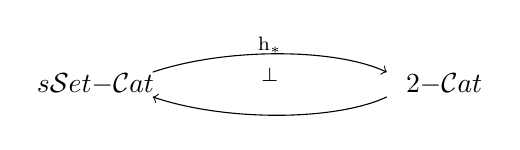
\begin{tikzpicture}[x=1.8em,y=1.4em]
  \node (sc) at (0,0) {$\sSet\text{-}\Cat$};
  \node (tc) at (7.0,0) {$2\text{-}\Cat$};
  \draw[->] (1.15,0.32) .. controls (2.6,0.95) and (4.8,0.95) .. (5.85,0.32);
  \node at (3.5,1.02) {$\scriptstyle\mathrm{h}_{*}$};
  \node at (3.5,0.25) {$\scriptstyle\bot$};
  \draw[->] (5.85,-0.32) .. controls (4.8,-0.95) and (2.6,-0.95) .. (1.15,-0.32);
\end{tikzpicture}
\end{center}
定义的换基伴随，它们在对象上的作用相同，而在 hom 上则分别施用%
\trHomotopyCategory{}函子或\trNerve{}函子。由
\cref{lem:change-of-base-underlying-categories}，右伴随——它从一个
2-\trCategory{}造出一个\trSimpliciallyEnrichedCategory——尊重底范畴：由对象
与 1-\trCell{}构成的底范畴，被等同于由对象与 0-箭头构成的底范畴。在此情形，
\trFunctor{} $\mathrm{h}\colon\sSet\to\Cat$ 与诸底集函子交换，故事实上两个伴
随都保持底范畴，这从直接计算也显而易见。特别地，一个\trInfinityCosmos{}的%
\trHomotopyTwoCategory{}具有相同的底 1-\trCategory。
\end{example}

\subsection*{练习}

\begin{exercise}\label{ex:monoidal-functors}
查阅幺半函子（monoidal functor）与幺半变换（monoidal transformation）的定义
——它们有时被称作\emph{松幺半函子}（lax monoidal functor）与\emph{松幺半变
换}（lax monoidal transformation）——并证明：
\begin{enumerate}[label=(\roman*)]
\item 带有限积的诸\trCategory{}之间的任何保持积的\trFunctor{}都是幺半的；并且
\item 这类\trFunctor{}之间的任何\trNaturalTransformation{}都是一个幺半自然
  变换。
\end{enumerate}
\end{exercise}

\begin{exercise}\label{ex:tensors-cotensors-underlying}
设 $\mathcal{V}$ 是一个\trCartesianClosed{}范畴，并设 $\mathcal{C}$ 是一个张
量化且余张量化的 $\mathcal{V}$-范畴。由
\cref{prop:change-of-base-tensored-cotensored}，底范畴 $\mathcal{C}_{0}$ 作为
一个非富集范畴是张量化且余张量化的。请描述这些张量与余张量。
\end{exercise}

